%    Template for seminar reports
% Seminar Current Topics in Computer Vision and Machine Learning
% Summer Semester 2015
% Computer Vision Group, Visual Computing Institute, RWTH Aachen

\documentclass[twoside,a4paper,article]{combine}


% =========================================================================
\usepackage[latin1]{inputenc}
\usepackage{a4}
\usepackage{fancyhdr}   
%\usepackage{german}    % Uncomment this iff you're writing the report in German
\usepackage{makeidx}
\usepackage{color}
\usepackage{t1enc}		% german letters in the "\hyphenation" - command
\usepackage{latexsym}	% math symbols
\usepackage{amssymb}    % AMS symbol fonts for LaTeX.

\usepackage{graphicx}
\usepackage{pslatex}
\usepackage{ifthen}

\usepackage[T1]{fontenc}
\usepackage{pslatex}

\usepackage{psfrag}
\usepackage{subfig}
\usepackage{url}

\usepackage{amsmath}
\usepackage{bm}

% =========================================================================

\setlength{\oddsidemargin}{3.6pt}
\setlength{\evensidemargin}{22.6pt}
\setlength{\textwidth}{426.8pt}
\setlength{\textheight}{654.4pt}
\setlength{\headsep}{18pt}
\setlength{\headheight}{15pt}
\setlength{\topmargin}{-41.7pt}
\setlength{\topskip}{10pt}
\setlength{\footskip}{42pt}

\setlength{\parindent}{0pt}

% =========================================================================

\graphicspath{
	{pictures/}
}

%%%
% We want also subsubsections to be enumerated
%%%
\setcounter{secnumdepth}{3}
\setcounter{tocdepth}{3}

\makeglossary
%\makeindex

% =========================================================================
\begin{document}

% Template for seminar reports
% Seminar Current Topics in Computer Vision and Machine Learning

\begin{titlepage}


\begin{center}
\ 
\vspace{3.5cm}


\textsf
{
Fakult�t f�r Mathematik, Informatik und Naturwissenschaften\\
Institude f�r Informatik II\\
Computer Graphik\\
Jun.Prof. Dr. Angela Yao
}

\rule{\linewidth}{1pt}

\vspace{1.75cm}
\LARGE
\textbf{Lab Report}

\vspace{1.7cm}
\huge
Unsupervised Learning of Video Representations using LSTMs

\vspace{3.0cm}
\Large
Cun Wang\\
\large
Matriculation Number: 362024

\vspace{0.5cm}
July 2017	

\vspace{1.05cm}
\rule{\linewidth}{1pt}

\vspace{0.5cm}
\textsf{\textbf{
\normalsize
\begin{tabular}{ll}
Advisor:  Moritz Wolter\\
\end{tabular}
}}
\end{center}

\end{titlepage}


\begin{abstract}
% +++++++++++++++++++++++++
% Insert your Abstract here
% +++++++++++++++++++++++++
In this lab, Long Short Term Memory (LSTM) networks are used to learn the representation of video sequences. It adpots the Encoder-Decoder
framework. An encoder LSTM is used to map the inputs sequences to a fixed length representation. Then an decoder LSTM decodes this
representation to reconstruct the input sequences. In order to capture spatiotemporal correlation better, the convolutional LSTM
(ConvLSTM) is applied besides fully-connected LSTM (FC-LSTM).

\end{abstract}

\tableofcontents
\newpage
% =========================================================================

% +++++++++++++++++++++++++
% Insert your Text here
% +++++++++++++++++++++++++

\section{Introduction}
Understanding temporal sequences is important for solving many problems, such as speech recognition, caption generation. Srivastava
\emph{et al.} use the LSTM Encoder-Decoder framework to learn video representations \cite{ulvr}. A sequence of frames are fed in encoder 
LSTM to generate a representation. This representation is then decoded through another LSTM to produce a target sequence. Srivastava
\emph{et al.} consider two choices of the target. One choice is to use the inputs as the target sequence. The other is to predict the
future frames. They also evaluate on two kinds of inputs. One is image patches, the other is the high-level "percepts" extracted by
applying a convolutional net.

LSTM is an important part of Encoder-Decoder framework. LSTM is a specical kind of recurrent neural network, which can capture long-term
temporal dependencies without suffering from the optimization problems such as gradient vanishing. In order to make use of frame structure,
convolutional LSTM introduced in \cite{convlstm} is applied in Encoder-Decoder framework.

\section{Methodology}
\subsection{LSTM architecture}
As mentioned above, Encoder-Decoder framework is composed of LSTMs. We'll introduce vanilla LSTM architecture \cite{odyssey}. A schematic
of the vanilla LSTM block is illustrated in figure \ref{fig:vanilla}. The key to LSTMs is the cell state, which is controlled by three
kinds of gates, adding information to or removing it from the cell state. The gates are composed of a sigmoid layer and a pointwise
multiplication operation. The output of sigmoid layer ranges from zero to one, describing how much of each component should be let through.
The forgate gate decides what information is going to be throwed away from the cell state. The input gate decides what information is going
to be stored in the cell state. The output gate decides what is going to output.
\begin{figure}
    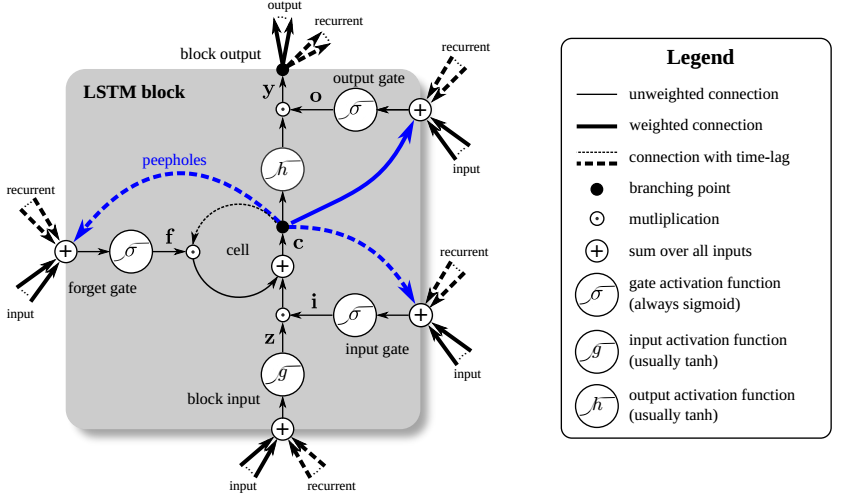
\includegraphics[width=\linewidth]{vanilla}
    \caption{vanilla LSTM block architecture}
    \caption*{Source: \protect\cite{odyssey}}
    \label{fig:vanilla}
\end{figure}

The vector formulas for a vanilla LSTM layer forward pass are given below. $\bm{x}^t$ is the input vector at time t, the $\bm{W}$ are 
rectangular input weight matrices, the $\bm{p}$ are peephole weight vectors and $\bm{b}$ are bias vectors. Functions $\sigma$, $g$ and 
$h$ are pointwise nonlinear activation functions. The pointwise multiplication of two vectors is denoted with $\odot$:

\subsection{Convolutional LSTM}
Video frames have spatio information in their structure, which is not captured by FC-LSTM, where full connections are used in
input-to-state and state-to-state transitions. To make use of saptio information, ConvLSTM is applied in this lab. In the ConvLSTM, the
inputs $\bm{X}_1,...\bm{X}_t$, cell outputs $\bm{C}_1,...\bm{C}_t$, hidden states $\bm{H}_1,...\bm{H}_t$, and gates $i_t,f_t,o_t$ are 3D
tensors whose last two dimensions are spatial dimensions (rows and columns). 

\begin{figure}[ht!]
    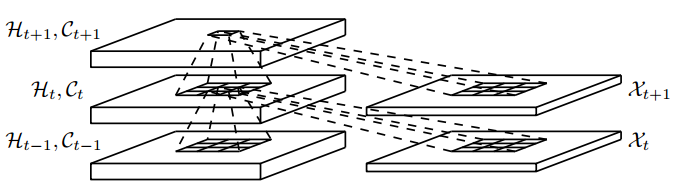
\includegraphics[width=\linewidth]{convlstm}
    \caption{inner structure of convolutional LSTM}
    \caption*{Source: adopted from slides of Kaiming He}
    \label{fig:convlstm}
\end{figure}

\subsection{LSTM autoencoder model}
This model is composed of two Recurrent Neural Network, the encoder LSTM and the decoder LSTM, as shown in figure \cite{fig:autoencoder}.
The input to the model is a sequence of vectors, in our case, video frames. The encoder LSTM runs through these frames to come up with a
representation, which is the state of encoder LSTM atfer the last frame has been read. The decoder LSTM then is expected to reconstruct
target seqence as input sequence based on the representation, which requires that representation contains information about the
appearance of the objects and the background as well as any motion in the video. Srivastava \emph{et al.} point out that it makes
optimization easier when target seqence is reversed compared to input sequence, because the model can look at low range correlation. 

\begin{figure}[ht!]
    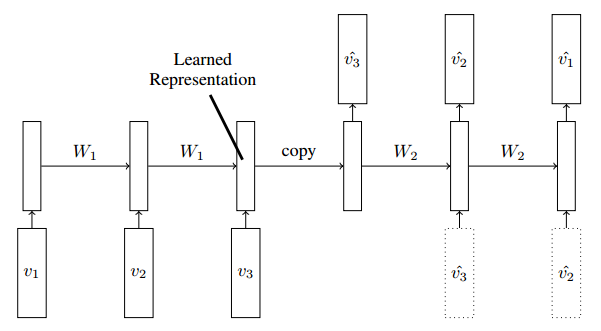
\includegraphics[width=\linewidth]{autoencoder}
    \caption{LSTM Autoencoder Model}
    \caption*{Source: adopted from slides of Kaiming He}
    \label{fig:autoencoder}
\end{figure}

\section{Experiments}
\subsection{Datasets}
The model is trained on a dataset of moving MNIST digits. Each video is 20 frames long and consist of 2 digits moving inside $64\times64$
patch.



% =========================================================================
\bibliographystyle{alpha}
\bibliography{lab_report}

% =========================================================================

\end{document}
